\section{Legendre Transform}

\subsection{Definition and Properties}

\begin{definition}[Legendre Transform]
    \label{def:legendre-transform}%
    The \emph{Legendre Transform} of \(\functiondomain{f}{\dom\pqty{f} \subseteq \RR^n}{\RR}\) is
    \[
        \legendre{f} \pqty{\vb{p}} = \sup_{\vb{x} \in \dom \pqty{f}} \bqty{\vb{p} \vdot \vb{x} - f\pqty{\vb{x}}}
    \]
    with its domain as \(\dom \pqty{\legendre{f}} = \set{\vb{p} \in \RR^n}{\text{the supremum exists and is finite}}\).
\end{definition}

\begin{proposition}[Legendre Transform is Convex]
    \label{prop:legendre-convex}%
    \(\legendre{f}\) is convex.
\end{proposition}

\begin{proof}
    Let \(\vb{p}, \vb{q} \in \dom \pqty{\legendre{f}}\), and \(t \in \oointv{0}{1}\). We note that
    \begin{align*}
        \sup_{\vb{x} \in \dom \pqty{f}} \Bqty{\bqty{\pqty{1 - t} \vb{p} + t \vb{q}} \cdot \vb{x} - f\pqty{\vb{x}}} &= \sup_{\vb{x} \in \dom \pqty{f}} \Bqty{\pqty{1 - t} \bqty{\vb{p} \vdot \vb{x} - f\pqty{\vb{x}}} + t \bqty{\vb{q} \vdot \vb{x} - f \pqty{\vb{x}}}} \\
        &\leq \pqty{1 - t} \sup_{\vb{x} \in \dom \pqty{f}} \pqty{\vb{p} \vdot \vb{x} - f\pqty{\vb{x}}} + t \sup_{\vb{x} \in \dom \pqty{f}} \pqty{\vb{q} \vdot \vb{x} - f\pqty{\vb{x}}}.
    \end{align*}

    Since the right-hand side is finite, so must be the left-hand side, and hence \(\pqty{1 - t} \vb{p} + t \vb{q} \in \dom \pqty{\legendre{f}}\). In particular, the previous inequality also showed that
    \[
        \legendre{f} \pqty{\pqty{1 - t} \vb{p} + t \vb{q}} \leq \pqty{1 - t} \legendre{f} \pqty{\vb{p}} + t \legendre{f} \pqty{\vb{q}}
    \]
    so \(\legendre{f}\) is indeed convex.
\end{proof}

\begin{proposition}
    \label{prop:dot-product-convex}%
    If \(f\) is convex, then so is
    \[
        F_{\vb{p}} \pqty{\vb{x}} = f\pqty{\vb{x}} - \vb{p} \vdot \vb{x}
    \]
    where \(\vb{p} \in \RR^n\) is fixed.
\end{proposition}

\begin{proof}
    We have \(\dom \pqty{F_{\vb{p}}} = \dom \pqty{f}\). Note
    \begin{align*}
        F_{\vb{p}} \pqty{\pqty{1 - t} \vb{x} + t \pqty{\vb{y}}} &= f\pqty{\pqty{1 - t} \vb{x} + t \vb{y}} - \vb{p} \vdot \pqty{\pqty{1 - t} \vb{x} + t \vb{y}} \\
        &\leq \pqty{1 - t} f \pqty{\vb{x}} + t f \pqty{\vb{y}} - \vb{p} \vdot f\pqty{\pqty{1 - t} \vb{x} + t \vb{y}} \\
        &= \pqty{1 - t} F_{\vb{p}} \pqty{\vb{x}} + t F_{\vb{p}} \pqty{\vb{y}}.
    \end{align*}
\end{proof}

\begin{corollary}[Legendre Transform of convex functions]
    \label{cor:legendre-transform-of-convex-function}
    If \(f\) is convex and differentiable, then any stationary point of \(\vb{p} \vdot \vb{x} - f \pqty{\vb{x}}\) (which is a concave function, by \autoref{prop:dot-product-convex}) is a global maximum occurring at \(\vb{x} \pqty{\vb{p}}\) given by solving
    \begin{equation}
        \grad f\pqty{\vb{x}} = \vb{p}.
        \label{eq:legendre-transform-of-convex-function}
    \end{equation}

    Hence, we have
    \[
        \legendre{f} \pqty{\vb{p}} = \vb{p} \vdot \vb{x} \pqty{\vb{p}} - f\pqty{\vb{x} \pqty{\vb{p}}}.
    \]
\end{corollary}

\begin{remark}
    If \(f\) is \emph{strictly} convex, then the solution to \autoref{eq:legendre-transform-of-convex-function} is unique. The idea is to consider the chord joining the two maxima of the function, and use the concave version of \autoref{eq:strict-convex-condition}.
\end{remark}

\begin{examples}[Legendre Transforms for \(n = 1\)]
    \label{ex:legendre-one-dimensional}%
    \begin{enumerate}
        \item Consider the quadratic \(f\pqty{x} = \frac{1}{2} a x^2\) for \(a > 0\). \(f\) is strictly convex, and \autoref{eq:legendre-transform-of-convex-function} holds if and only if \(x = \flatfrac{p}{q}\). Hence,
        \[
            \legendre{f} \pqty{p} = \frac{p^2}{a} - \frac{p^2}{2a} = \frac{p^2}{2a}.
        \]
        
        This is indeed convex, with domain \(\RR\).

        \item Consider the function \(f\pqty{v} = - \sqrt{1 - v^2}\) defined for \(-1 < v < 1\). This is a semi-circle and is convex. \autoref{eq:legendre-transform-of-convex-function} holds if and only if \(p = \flatfrac{v}{\sqrt{1 - v^2}}\). This gives the solution
        \[
            v = \frac{p}{\sqrt{1 + p^2}}
        \]
        for \(p \in \RR\). Hence,
        \[
            \legendre{f} \pqty{p} = \frac{p^2}{\sqrt{1 + p^2}} + \frac{1}{\sqrt{1 + p^2}} = \sqrt{1 + p^2},
        \]
        and this is defined for \(p \in \RR\).

        \autoref{fig:graph-legendre-one-dimensional-2} are the graphs for the two functions.

        \item Let \(f\pqty{x} = cx\) for \(c > 0\). This is a convex function, but not strictly convex. The domain is given by \(\dom\pqty{f} = \RR\), and note
        \[
            px - f\pqty{x} = \pqty{p - c} x.
        \]

        If \(p \neq c\), the supremum of this is infinite (since \(x\) can be arbitrarily large in both directions). This supremum only exists for \(p = c\), and hence
        \[
            \legendre{f}\pqty{p} = 0
        \]
        only defined for \(p = c\), i.e. \(\dom \pqty{\legendre{f}} = \Bqty{c}\).
    \end{enumerate}
\end{examples}

\begin{figure}[ht!]
    \centering
    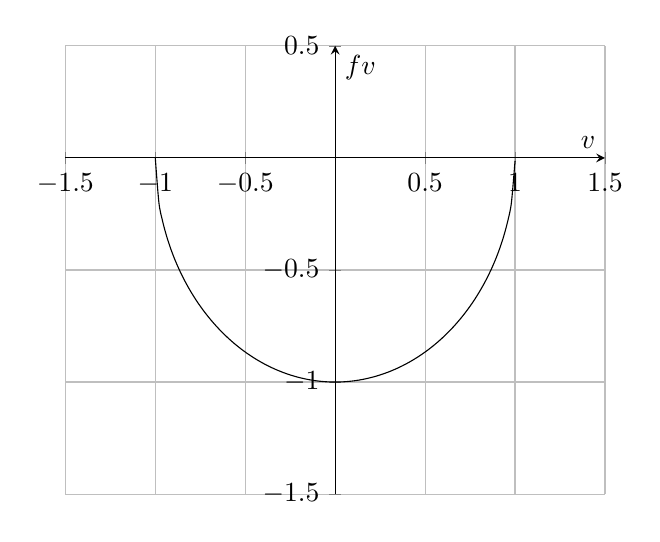
\begin{tikzpicture}[scale=1]
        \begin{axis}[grid=both,
                     xmin=-1.5, xmax=1.5, xlabel=\(v\),
                     ymin=-1.5, ymax=0.5, ylabel=\(f\pqty{v}\),
                    axis lines=center, >=stealth]
        \addplot[domain=-1:1, samples=100] plot[smooth] {- sqrt(1 - x^2)};
        \end{axis}
    \end{tikzpicture}


    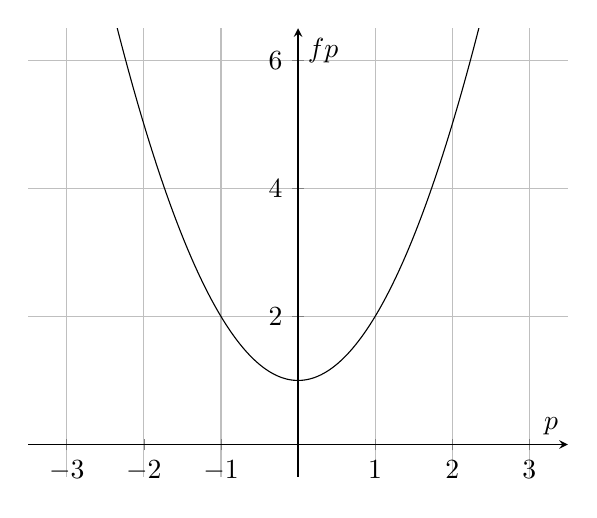
\begin{tikzpicture}[scale=1]
        \begin{axis}[grid=both,
                     xmin=-3.5, xmax=3.5, xlabel=\(p\),
                     ymin=-0.5, ymax=6.5, ylabel=\(\legendre{f}\pqty{p}\),
                    axis lines=center, >=stealth]
        \addplot[domain=-3:3, samples=100] plot[smooth] {sqrt{1 + x^2}};
        \end{axis}
    \end{tikzpicture}
    \caption{Graph for \autoref{ex:legendre-one-dimensional} (2)}
    \label{fig:graph-legendre-one-dimensional-2}
\end{figure}

What happens if we do a Legendre transform twice?

\begin{theorem}[Legendre Transform of Legendre Transform for Convex Functions]
    \label{thm:legendre-transform-of-legendre-transform}%
    If \(f\) is convex and \(\contClass{2}\), then \(\llegendre{f} = f\).
\end{theorem}

\begin{proof}
    To find \(\llegendre{f}\), we need to find \(\vb{p} \pqty{\vb{x}}\) obeying \autoref{eq:legendre-transform-of-convex-function}, u.e.,
    \[
        \grad \legendre{f} \pqty{\vb{p} \pqty{\vb{x}}} = \vb{x} \eqno{(\ast)}
    \]

    Note that
    \[
        \legendre{f} \pqty{\vb{p}} = \vb{p} \vdot \vb{x} \pqty{\vb{p}} - f\pqty{\vb{x} \pqty{\vb{p}}}
    \]
    where \(\vb{x} \pqty{\vb{p}}\) is given by \autoref{eq:legendre-transform-of-convex-function}.

    Differentiating \(\legendre{f}\) with respect to \(\vb{p}\), we have
    \begin{align*}
        \pdv{\legendre{f}}{p_i} &= x_i + p_j \pdv{x_j}{p_i} - \pdv{x_j}{p_i} \pdv{f}{x_j}\pqty{\vb{x}\pqty{\vb{p}}} && \text{allowed by smoothness assumption of \(f\)} \\
        &= x_i + \pdv{x_j}{p_i} \pqty{p_j - \nabla_j f \pqty{\vb{x} \pqty{\vb{p}}}} \\
        &= x_i. && \text{by \autoref{eq:legendre-transform-of-convex-function}}
    \end{align*}

    So we have
    \[
        \grad \legendre{f} \pqty{\vb{p}} = \vb{x} \pqty{\vb{p}}.
    \]

    So \((\ast)\) reduces to \(\vb{x} \pqty{\vb{p} \pqty{\vb{x}}} = \vb{x}\), which means that \(\vb{x}\pqty{\vb{p}}\) is the inverse of \(\vb{p} \pqty{\vb{x}}\).

    So
    \begin{align*}
        \llegendre{f} \pqty{\vb{x}} &= \vb{x} \vdot \vb{p} \pqty{\vb{x}} - \legendre{f} \pqty{\vb{p} \pqty{\vb{x}}} \\
        &= \vb{x} \vdot \vb{p} \pqty{\vb{x}} - \pqty{\vb{p} \pqty{\vb{x}} \vdot \vb{x} - f \pqty{\vb{x} \pqty{\vb{p} \pqty{\vb{x}}}}} \\
        &= f\pqty{\vb{x}}.
    \end{align*}
\end{proof}

\begin{remark}
    Obviously, \(f\) is convex is necessary since for the equation to hold, \(f\) is the Legendre transform of something, hence convex. But the \(\contClass{2}\) condition can be weakened significantly.
\end{remark}

\begin{example}[Double Legendre Transform of the Line]
    We note that
    \[
        \llegendre{f} \pqty{x} = \sup_{p \in \Bqty{c}} \pqty{xp - \legendre{f} \pqty{p}} = cx = f\pqty{x}
    \]
    indeed.
\end{example}

\subsection{Application of Legendre Transforms in Thermodynamics}

An important application of Legendre transforms is in thermodynamics.

Consider a system made of many molecules (say \(10^{23}\)). We are concerned with the \emph{macroscopic} behaviour of the system, i.e., involving length scale \(\gg\) separation of molecules.

In \emph{thermal equilibrium}, we may describe the macroscopic physics of the system by just a few quantities: total energy \(E\), volume \(V\), temperature \(T\), pressure \(p\), and perhaps some others.

An \emph{isolated system} is one which is simply not interacting with anything else, for example a gas in a vacuum flask.

In thermal equilibrium, macroscopic physics in gas in a vacuum flask is \textbf{fully specified} by two quantities, \(E\) and \(V\). However, microscopically, this is far away from the description in microscopic physics (since we need to specify the position, velocity, orientation, etc. of each microscopic molecule). Therefore, there is some number of \(\Omega \pqty{E, V}\) of microscopic configurations that ``look identical'' macroscopically, at the scale of
\[
    \Omega \sim 10^{10^{23}}
\]

\begin{definition}[Entropy]
    We define the \emph{entropy} as
    \begin{equation}
        \label{eq:entropy}%
        S\pqty{E, V} = k_{\text{B}} \log \Omega \pqty{E, V},
    \end{equation}
    where \(k_{\text{B}} = \SI{1.38 e-23}{\joule\per\kelvin}\) is the Boltzmann constant.
\end{definition}

If energy increased at fixed volume, then entropy will go up, because there are more ways to partition \(E\) between the molecules. This means \(S\) is strictly increasing with \(E\), and hence invertible to define
\begin{equation}
    \label{eq:energy}%
    E = E \pqty{S, V}.
\end{equation}

\begin{definition}[Temperature, Pressure]
    We may define the \emph{temperature} and \emph{pressure} as
    \begin{subequations}
        \label{eq:temperature-pressure}%
        \begin{equation}
            \label{eq:temperature}%
            T = \pqty{\pdv{E}{S}}_{V} > 0
        \end{equation}
        \begin{equation}
            \label{eq:pressure}%
            P = - \pqty{\pdv{E}{V}}_{S}
        \end{equation}
    \end{subequations}
    respectively.
\end{definition}

\begin{proposition}[Fundamental Thermodynamic Relation]
    We have
    \begin{equation}
        \label{eq:fundamental-thermodynamic-relation}%
        \dd{E} = p \dd{S} - P \dd{V}
    \end{equation}
\end{proposition}

What is below is an overview of the Legendre Transforms -- details can be found on Example Sheets.

\begin{example}[Legendre Transforms for Temperature -- Helmholtz Free Energy]
    Now, we forget \autoref{eq:temperature} (for temperature). Consider the Legendre Transform of \(E\pqty{S, V}\) with respect to \(S\), with parameter \(T\). Call this \(-F\), i.e.,
    \[
        -F \pqty{T, V} = \sup_{S} \Bqty{TS - E \pqty{S, V}}.
    \] 

    We may show that the stability of equilibrium state implies that \(E\) is convex, with respect to \(S\). Now, \autoref{eq:legendre-transform-of-convex-function} maximises for \(S\pqty{T, V}\) satisfying \autoref{eq:temperature}, and
    \[
        F\pqty{T, V} = E - TS
    \]
    is called the \emph{Helmholtz Free Energy}.

    Note \autoref{eq:fundamental-thermodynamic-relation} implies that
    \[
        \dd{F} = - S \dd{T} - P \dd{V}
    \]
    and hence
    \begin{align*}
        S &= - \pqty{\pdv{F}{T}}_{V}, \\
        P &= - \pqty{\pdv{F}{V}}_{T}.
    \end{align*}

    In Part II, we will see that \(F\) is useful when considering an \emph{non-isolated} system in equilibrium with an \emph{enviroment} ad temperature \(T\), for example gas in an uninsulated box.
\end{example}

\begin{example}[Legendre Transforms for Pressure -- Enthalpy]
    Similarly, we forget \autoref{eq:pressure} (for pressure). Consider the Legendre Transform of \(E\pqty{S, V}\) with respect to \(V\) at fixed \(S\), with parameter \(-P\). We call this \(-H\), i/e/,
    \[
        -H \pqty{S, P} = \sup_{V} \Bqty{- {V - E \pqty{S, V}}}
    \]

    Similarly, applying \autoref{eq:legendre-transform-of-convex-function} maximises for \(V\) satisfying \autoref{eq:pressure}, and
    \[
        H\pqty{S, P} = E + PV
    \]
    is called the \emph{enthalpy}. It is very useful in chemistry.

    Now, \autoref{eq:fundamental-thermodynamic-relation} implies that
    \[
        \dd{H} = T \dd{S} + V \dd{P}
    \]
    and hence
    \begin{align*}
        T &= \pqty{\pdv{H}{S}}_{P}, \\
        V &= \pqty{\pdv{H}{P}}_{S}.
    \end{align*}
\end{example}

\begin{example}[Legendre Transforms for Both -- Gibbs Free Energy]
    Finally, we may take the Legendre transform of \(E \pqty{S, V}\) with respect to both \(S\) and \(V\) with parameters \(T, -P\), and call this \(-G\). (This is same as Legendre Transform of \(F\) w.r.t. \(V\), or \(H\) w.r.t. \(S\).) We have
    \[
        -G \pqty{T, P} = \sup_{S, V} \Bqty{TS - PV - E \pqty{S, V}}
    \]
    and applying \autoref{eq:legendre-transform-of-convex-function}, we have the maximum of \(S\pqty{T, P}\) and \(V\pqty{T, P}\) gives both of \autoref{eq:temperature-pressure}. Hence, \(G\) is given by
    \[
        G\pqty{T, P} = E - TS + PV
    \]
    is called the \emph{Gibbs free energy}.

    Using \autoref{eq:fundamental-thermodynamic-relation} gives
    \[
        \dd{G} = -S \dd{T} + V \dd{P}
    \]
    and hence
    \begin{align*}
        S &= - \pqty{\pdv{G}{T}}_{P}, \\
        V &= \pqty{\pdv{G}{P}}_{T}.
    \end{align*}
\end{example}

\begin{definition}[Thermodynamic Potentials]
    \(E, F, G, H\) are called \emph{thermodynamic potentials}.
\end{definition}

Assuming that everything is \(\contClass{2}\), we have
\[
    \pdv{E}{S}{V} = \pdv{E}{V}{S},
\]
and hence
\[
    \pqty{\pdv{S} \pqty{\pdv{E}{V}}_S}_{V} = \pqty{\pdv{V} \pqty{\pdv{E}{S}}_{V}}_{S}.
\]

Applying \autoref{eq:temperature-pressure} gives
\[
    - \pqty{\pdv{P}{S}}_{V} = \pqty{\pdv{T}{V}}_{S}
\]

There are three similar equations that follow from doing the same steps with different thermodynamic potentials, from \(F, H\) and \(G\).

\begin{definition}[Maxwell Relations]
    The four equations derived from the four thermodynamic potentials are the \emph{Maxwell relations}.
\end{definition}